\documentclass[9pt]{beamer}
% \documentclass[notes, handout, 9pt]{beamer}
% \documentclass[handout, 9pt]{beamer}

\usepackage{import}
\subimport{../}{preamble.tex}
\subimport{../}{beamer-theme.tex}
\usepackage{svg}

% Location for all figures / pictures
\graphicspath{{pictures/}{figures/}}

% % Figures inline
\usepackage{tikz}
\usetikzlibrary{arrows,positioning}
\usetikzlibrary{calc}

\usepackage{pgfplots}
%--------------------------------------------------
% Presentation Information
%--------------------------------------------------
\title[Continuous Optimization]{Gradient Descent and Subgradients}
\author[]{\textbf{Bart Van Parys}}
\date[]{Fall 2026}
%--------------------------------------------------

\begin{document}

\begin{frame}  

  \maketitle

  \vspace{-2em}
  
    \begin{center}
    \begin{tabular}{lll}
      Instructor : & \textbf{Bart Van Parys} & \textbf{(\href{mailto:mastermath@vanparys.xyz}{mastermath@vanparys.xyz})} \\
    \end{tabular}
  \end{center}
  
\end{frame}

\section{Differentiability}

\begin{frame}{A Brief Recall of Differentiability}


  Let $f:\Re^n\to\nRe$ be continuous.

  \begin{enumerate}
    \setlength\itemsep{2em}
  \item The function $f$ is \emph{directionally differentiable} at $x \in \dom(f)$ in the direction $d$ if the following limit exists:
    \[
      \nabla f(x)[d] = \lim_{t\downarrow 0} \frac{f(x+t d)-f(x)}{t}.
    \]
  \item<2-> The function $f$ is (G\^ateaux) \emph{differentiable} in $x \in \dom(f)$ if differentiable in $x$ in every direction $d \in \Re^n$ and if the directional derivative is linear in the direction, i.e.,
    \[
      \nabla f(x)[d] = \iprod{f'(x)}{d} = f'(x)\tpose d  \qquad\forall d \in \Re^n.
    \]
    The vector $f'(x)$ is called the gradient at $x$.
  \item<3-> $f$ is \emph{continuously differentiable} if $x \mapsto f'(x)$ is continuous

  \item<4-> $f$ is \emph{smooth} if $x \mapsto f'(x)$ is Lipschitz
  \end{enumerate}
  
  
\end{frame}

\begin{frame}{Examples}

  \begin{minipage}{0.6\textwidth}
    \includegraphics[height=2.25cm]{not-dir-deriv/function.pdf}
  \end{minipage}%
  \hfill
  \begin{minipage}{0.4\textwidth}
    Continuous.\\
    Not directionally differentiable.
  \end{minipage}
  
  \vfill

  \begin{minipage}{0.6\textwidth}
    \includegraphics[height=2.25cm]{dir-deriv/function.pdf}
  \end{minipage}%
  \hfill
  \begin{minipage}{0.4\textwidth}
    Directionally differentiable.\\
    Not differentiable.
  \end{minipage}
  
  \vfill

  \begin{minipage}{0.6\textwidth}  
    \includegraphics[height=2.25cm]{deriv/function.pdf}
  \end{minipage}%
  \hfill
  \begin{minipage}{0.4\textwidth}
    (Continuously) differentiable.\\
  \end{minipage}


\end{frame}


\section{Smooth Nonlinear Optimization}

\begin{frame}{Nonlinear Optimization}

  Let $f:\Re^n\to\Re$ be a continuously differentiable function. We would like to find a minimizer $x^\star$ of the unconstrained problem
  \[
    \begin{array}{rl}
      \minimize & f(x) \\[1em]
      \st & x \in \Re^n.
    \end{array}
  \]
    
  \vfill

  \textbf{Too much to ask for!}
  \begin{itemize}
  \item<2-> We will settle for finding any stationary point $\bar x$ with $f'(\bar x)=0$.
  \item<2-> When $f$ is convex $\bar x$ is a minimizer.
  \end{itemize}

  \vfill

  \uncover<3->{
  \textbf{Theorem : } Suppose that $f$ is continuously differentiable and there exists a minimizer $x^\star \in \interior(\dom(f))$. Then, $f'(x^\star) = 0$.
}
\end{frame}

\begin{frame}{Gradient Descent}

  
  \begin{algorithm}[H]
    \SetKwInput{Initialization}{Initialisation}
    \Initialization{$x_0$ feasible}
    \For{$k\geq 0$}{
      $x_{k+1} \defn x_k - h_k f'(x_k)$
    }
    \caption{Gradient Descent}
  \end{algorithm}

  \vfill
  
  \emph{Gradient method} proceeds in the steepest descent direction.
  \begin{itemize}
  \item How to choose step sizes $(h_k)_{k\geq 0}>0$?
  \end{itemize}

  \vfill

  \uncover<2->{
    In machine learning $(h_k)_{k\geq 0}>0$ are called \emph{learning rates}.
  }
\end{frame}

\begin{frame}{Stationary Points}

  \begin{center}
    \includegraphics[height=5cm]{stationary-point/stationary-point.pdf}
  \end{center}
  
  \vfill
  
  \textbf{Example:}
  \[
    f(x_1, x_2) = \frac12 x_1^2 + \frac14 x_2^4-\frac12 x_2^2 
  \]

  \vfill

  \begin{itemize}
  \item Stationary points  are
    $s_1 = (0, 0)$, $s_2=(0, -1)$ and $s_3=(0, 1)$
  \item<2-> Only $s_2$ and $s_3$ are minima.
  \item<3-> If $x_0=(1, 0)$ then gradient descent with $f'(x_1, x_2) = (x_1, -x_2+x_2^3)$ converges to $s_1$!
  \end{itemize}
  
\end{frame}


\begin{frame}{Smooth Optimization}
  
  \textbf{Smoothness Assumption :} $f$ has \emph{Lipschitz continuous gradient}, or is smooth, i.e., $\exists L>0$ such that
  \[
    \norm{f'(x)-f'(y)}_\star \leq L\norm{y-x}\quad \forall x, y\in \dom(f)
  \]

  We call such a function $L$-smooth w.r.t.\ $\norm{\cdot}$, or $L$-smooth if the norm is clear from context.

  \vfill

  \textbf{Remark:}
  \begin{itemize}
  \item Dual norm $\norm{u}_\star = \sup \set{\iprod{u}{x}}{\norm{x}\leq 1}$.
  \item The Euclidean norm is self-dual $\norm{x}_{2, \star} = \norm{x}_2$.
  \item More on dual norms later.
  \end{itemize}
\end{frame}


\begin{frame}{Geometric interpretation}

  \begin{center}
    \includegraphics[height=6cm]{smooth-function/smooth-function.pdf}
  \end{center}
  
\end{frame}

\begin{frame}{Geometric Interpretation}

  \textbf{Theorem :} Let $f$ be $L$-smooth w.r.t.\ $\norm{\cdot}$. Then,
  \[
    \abs{f(y)-f(x)-\iprod{f'(x)}{y-x}} \leq \frac{L}{2} \norm{y-x}^2 \quad \forall x, y\in \dom(f)
  \]

  \vfill

  \textbf{Proof [$\star$]: }
  \[
    \begin{array}{rlr}
      & \abs{f(y)-f(x)-\iprod{f'(x)}{y-x}} & \\[1em]
      = & \abs{\int_{0}^1 \iprod{f'(x+t(y-x))-f'(x)}{y-x} \d t} & \\[1em]
      \leq & \int_0^1 \norm{f'(x+t(y-x))-f'(x)}_\star \d t \norm{y-x} & [Cauchy-Schwarz]\\[1em]
      \leq & L \int_0^1 t \d t \norm{y-x}^2 & [L-Smoothness]\\[1em]
      \leq & \frac{L}{2} \norm{y-x}^2 & 
    \end{array}
  \]
\end{frame}

\begin{frame}{Gradient Method Converges with Fixed Step-Size}

  \textbf{Theorem:} Let $f$ be $L$-smooth and $-\infty < p^\star = \inf_{x\in\Re^n} f(x)$. The gradient method with step-size $0<h_k = \eta < \frac{2}{L}$ converges to a stationary point.

\end{frame}

\begin{frame}{Proof}

  \textbf{Proof:}
  \begin{itemize}
  \item We have that
    \begin{align*}
      f(x_{k+1}) \leq &  f(x_k) + \iprod{f'(x_k)}{x_{k+1}-x_k} + \frac{L}{2} \norm{x_{k+1}-x_k}^2 \\
      \leq & f(x_k) - \eta \norm{f'(x_k)}^2+\frac{\eta^2 L}{2} \norm{f'(x_k)}^2 \\
      \leq & f(x_k) - \eta (1-\frac{\eta}{2}L)\norm{f'(x_k)}^2
    \end{align*}
    because $f$ is $L$-smooth and $x_{k+1} - x_k = - \eta f'(x_k)$.
  \item<2-> Hence, we have that $\norm{f'(x_k)}^2\leq 1/(\eta (1-\frac{\eta}{2}L)) (f(x_k)-f(x_{k+1}))$.
  \item<3-> By telescoping the previous inequality we get for all $n\geq 1$ that
    \[
      \sum_{k=0}^{n-1} \norm{f'(x_k)}^2 \leq 1/(\eta (1-\tfrac{\eta L}{2}))\cdot (f(x_0)-f(x_{n})) \leq (f(x_0)-p^\star)/(\eta (1-\tfrac{\eta L}{2})) 
    \]
    and hence $\lim_{n\to\infty} \norm{f'(x_n)}=0$.
  \end{itemize}
  
\end{frame}

\begin{frame}{Rate of Convergence}

  \begin{itemize}
  \item Let $g^\star_n=\min_{k\in [0, \dots, n-1]} \norm{f'(x_k)}$. We have $n\cdot (g_n^\star)^2\leq \sum_{k=0}^{n-1} \norm{f'(x_k)}^2$ and hence
    \[
      g_n^\star \leq \frac{\sqrt{f(x_0)-p^\star}}{\sqrt{n}}\cdot 1/\sqrt{\eta (1-\tfrac{\eta L}{2})}
    \]
  \end{itemize}
  
\end{frame}


\begin{frame}{Optimal Fixed Step-Size}

  \begin{algorithm}[H]
    \SetKwInput{Initialization}{Initialisation}
    \Initialization{$x_0$ feasible}
    \For{$k\geq 0$}{
      $x_{k+1} \defn x_k - \eta f'(x_k)$
    }
    \caption{Gradient Descent}
  \end{algorithm}

  \vfill
  
  Descent method when $0<\eta<\tfrac{2}{L}$ as
  \[
    f(x_{k+1}) \leq  f(x_k) - \eta (1-\tfrac{L \eta}{2})\norm{f'(x_k)}^2<f(x_{k}).
  \]

  \vfill

  Choose step size $\eta^\star$ which maximizes the descent lower bound
  \begin{align*}
    \eta^\star \in & \arg\max_{\eta} ~\eta(1-\tfrac{L \eta}{2})\\
    = & ~\frac{1}{L}.
  \end{align*}
  
\end{frame}

\begin{frame}{What happens if the step length is not $\frac{1}{L}$}

  \begin{minipage}{0.5\textwidth}
    \center
    \includegraphics[height=4cm]{gradient-descent/gradient-descent-L-too-small.pdf}\\[1em]
    \emph{$h_k = \frac{1}{L}-\delta$}
  \end{minipage}%
  \hfill
  \begin{minipage}{0.5\textwidth}
    \center
    \includegraphics[height=4cm]{gradient-descent/gradient-descent-L-too-big.pdf}\\[1em]
    \emph{$h_k = \frac{1}{L}+\delta$}
  \end{minipage}
  
\end{frame}

\begin{frame}{Gradient Descent with Exact Line Search}

  \begin{algorithm}[H]
    \SetKwInput{Initialization}{Initialisation}
    \Initialization{$x_0$ feasible}
    \For{$k\geq 0$}{
      $h_k \in \arg\min_{t\geq 0} f(x_k-t f'(x_k))$\\
      $x_{k+1} \defn x_k - h_k f'(x_k)$
    }
    \caption{Gradient Descent}
  \end{algorithm}

  \vfill

  \textbf{Theorem:} Let $f$ be $L$-smooth and $-\infty < p^\star = \inf_{x\in\Re^n} f(x)$. The gradient method with exact line search converges to a stationary point.
  
  \textbf{Proof:} Exactly the same as before, as the descent
  \[
    f(x_{k+1}) \leq  f(x_k) - \frac{\norm{f'(x_k)}^2}{2L},
  \]
  is at least as fast as optimal fixed step-size.

  \vfill

  \uncover<2->{
    \textbf{Crucial point:} we do not need to know $L$ in the \emph{algorithm}!
  }
  
\end{frame}

\begin{frame}{Exact Line Search}

  At each iteration we must solve
  \[
    h_k \in \arg\min_{t\geq 0} ~g(t)\defn f(x_k-t f'(x_k)).
  \]

  \vfill

  \begin{center}
    \includegraphics[height=4cm]{line-search/line-search.pdf}
  \end{center}

  \textbf{Observations:}
  \begin{itemize}
  \item Requires solving a one dimensional optimization problem.
  \item May not be practical.
  \end{itemize}
  
\end{frame}

\begin{frame}{Wolfe Conditions}

  \begin{center}
    \includegraphics[height=4cm]{wolfe-conditions/wolfe-condition.pdf}
  \end{center}

  \vfill

  The step size $\bar t$ satisfies the \emph{Wolfe conditions} if
  \[
    \begin{array}{r@{\hspace{2em}}l}
      g(\bar t) \leq g(0) + \alpha \bar t g'(0) & [{\rm{Sufficient~decrease}}]\\[1em]
      g'(\bar t) \geq \beta g'(0) & [{\rm{Sufficient~progress}}]
    \end{array}
  \]
  for some $0 < \alpha < \beta < 1$ and where $g(t)\defn f(x-t f'(x))$.   
\end{frame}

\begin{frame}{Existence of Proper Step Sizes}

  Let $W_{\alpha, \beta}(x)$ be the set of all step sizes $\bar t$ which satisfy the Wolfe conditions at $x$.

  \vfill
  
  \textbf{Theorem:} Let $f:\Re^n\to\Re$ be continuously differentiable with $-\infty < p^\star =\inf_{x\in\Re^n}~f(x)$. Then, the set of step sizes $W_{\alpha, \beta}(\bar x)$ at any nonstationary point $\bar x$ has nonempty interior.

  \vfill
  
  \textbf{Algorithms:} There are efficient algorithms to find points in $W_{\alpha, \beta}(\bar x)$ efficiently.
\end{frame}

\begin{frame}{Proof [$\star$]}

  \textbf{Proof:} We have that $f'(\bar x)\neq 0$ and hence $g'(t) = -\iprod{f'(\bar x-t f'(\bar x))}{f'(\bar x)}$ and $g'(0)<0$. Let $d(t)\defn g(t)-g(0)-\alpha t g'(0)$. Then, $d'(0)=g'(0)(1-\alpha)<0$.
  By continuity of $f'$ there exists a $T>0$ such that $d'(t)<0$ for all $t\in [0, t']$ with $0<t'\leq T$. By the \emph{MVT}, there is an $\bar t \in (0, t')$ such that
  \[
    d(t')-d(0) =  t' d'(\bar t) <0.
  \]
  Hence, $d(t')<d(0)$ for all $t'\in(0,T)$. Note that $g(t)$ is bounded from below for all $t> 0$ while $g(0)-\alpha t g'(0)$ with $\alpha>0$ is not. Hence, we may take
  \[
    0 < T \leq t_a = \min \set{t>0}{d(t)=d(0)=0}.
  \]
  All step sizes $\bar t \in (0, t_a)$ evidently satisfy the sufficient decrease condition. The \emph{MVT} guarantees $d(t_a)-d(0)=t_a d'(t_b) = 0$ for some $t_b \in (0, t_a)$. Hence, $d'(t_b) = g'(t_b)-\alpha g'(0)=0$ and thus $g'(t_b)>\beta g'(0)$ as $\alpha < \beta$ and $g'(0)<0$. All step sizes $\bar t \in (t_b, t_a)$ with $0<t_b<t_a$ satisfy both Wolfe conditions.


\end{frame}

\begin{frame}{Inexact Line Search}

  \begin{algorithm}[H]
    \SetKwInput{Initialization}{Initialisation}
    \Initialization{$0<\alpha<\beta<1$ and $x_0$ feasible}
    \For{$k\geq 0$}{
      $h_k \in W_{\alpha, \beta}(x_k)$\\
      $x_{k+1} \defn x_k - h_k f'(x_k)$
    }
    \caption{Gradient Descent}
  \end{algorithm}

  \vfill
  
  \textbf{Theorem:} Let $f$ be $L$-smooth and $-\infty < p^\star = \inf_{x\in\Re^n} f(x)$. The gradient method with any step size satisfying the Wolfe conditions converges to a stationary point.

  \vfill
  
  \uncover<2->{
  \textbf{Proof [$\star$]:} We have using Cauchy-Schwarz and  $L$ smoothness that
  \(
    \iprod{f'(x_{k+1})-f'(x_k)}{-f'(x_k)} \leq \norm{f'(x_{k+1})-f'(x_k)}_\star\norm{f'(x_k)} 
    \leq L \norm{x_{k+1}-x_k}\norm{f'(x_k)} \leq L h_k \norm{f'(x_k)}^2
    \). From the second Wolfe condition we have that \(\iprod{f'(x_{k+1})-f'(x_k)}{-f'(x_k)} \geq (1-\beta)\norm{f'(x_k)}^2\) and hence $h_k \geq (1-\beta)/L$. The first Wolfe condition guarantees hence
    \[
      f(x_{k+1}) \leq f(x_k)-\frac{\alpha(1-\beta)}{L} \norm{f'(x_k)}^2.
    \]
    Remainder of the proof is the same as before.
    }
\end{frame}

\begin{frame}{Backtracking}

  \begin{center}
    \includegraphics[height=4cm]{wolfe-conditions/wolfe-condition.pdf}
  \end{center}

  \vfill

  Instead of the sufficient progress condition we can determine $\bar t$ also using backtracking
  \[
    \begin{array}{r@{\hspace{2em}}l}
      g(\bar t) \leq g(0) + \alpha \bar t g'(0) & [{\rm{Sufficient~decrease}}]\\[1em]
      \gray{g'(\bar t) \geq \beta g'(0)} & \gray{[{\rm{Sufficient~progress}}]}
    \end{array}
  \]
  for some $0 < \alpha \gray{< \beta} < 1$ and where $g(t)\defn f(x-t f'(x))$.   
\end{frame}

\begin{frame}{Backtracking}

  \begin{algorithm}[H]
    \SetKwInput{Initialization}{Initialisation}
    \Initialization{Choose $t_{\max}>0$, $\rho\in(0,1)$, $\bar t=t_{\max}$ }
    \While{$g(\bar t) > g(0) + \alpha \bar t g'(0)$}{
      $\bar t \defn \rho \cdot \bar t$
    }
    \caption{Backtracking}
  \end{algorithm}
  
\end{frame}

\section{Subgradients}

\begin{frame}{Differentiable Convex Functions}

  Let $f:\Re^n\to\nRe$ be a differentiable convex function. For any two points $x, y\in\dom(f)$ we have
  \begin{align*}
    \iprod{f'(x)}{y-x} & = \lim_{t\to 0} \frac{f(x + t(y-x))-f(x)}{t} \\
                       & \leq \lim_{t\to 0} \frac{(1-t)f(x) + t f(y)-f(x)}{t} = f(y) - f(x).
  \end{align*}
  
  \vfill
  \textbf{Gradient Property :}
  \[
    f(y) \geq f(x) + \iprod{f'(x)}{y-x} \quad \forall x, y\in\dom(f).
  \]

  \vfill

  \begin{center}
    \begin{tikzpicture}
      \draw[draw=blue, thick] plot[id=ex1,domain=-4:4,samples=1000] function {cosh(0.4*x)};
      % \fill[blue!5] plot[id=ex2,domain=-4:4,samples=1000] function {cosh(0.4*x)} -- (4, 3) -- (-4, 3) -- cycle;

      \node[above] at ($(4, {cosh(0.4*4)})+(-0.4, -0.1)$) {\color{blue} $f$};
      
      \draw[->] (-4, 0) -- (4, 0);
      \node[right] at (4, 0) {$\Re^n$};
      % \node[above] at (-4, 3) {$\Re_+$};
      \draw[->] (-4, 0) -- (-4, 3);

      % Lazy constraint 1
      \def\sa{-2}
      \fill[red] (\sa, 0) circle [radius=2pt];
      \draw[densely dotted, <->] (\sa, 0) -- ($(\sa, {cosh(0.4*\sa)})$);
      \draw[draw=red,line width=0.2mm] plot[id=lc1,domain=-4:1.5,samples=1000] function {0.4*sinh(0.4*\sa)*(x-\sa)+cosh(0.4*\sa)};
      \uncover{\node[below] at (\sa, -.1) {\red{$x$}};}
    \end{tikzpicture}
  \end{center}

\end{frame}

\begin{frame}{Subgradients of Convex Functions}


  \begin{minipage}{0.65\textwidth}
    We denote the set
    \[
      \partial f(x_0) \defn \set{g{\rm{~linear}}\!}{\!f(x) \geq f(x_0)+ g(x-x_0)~ \forall x\in \Re^n}
    \]
    as the \emph{subdifferential} of $f$ at $x_0$.
  \end{minipage}%
  \hfill
  \begin{minipage}{0.35\textwidth}
    \centering
    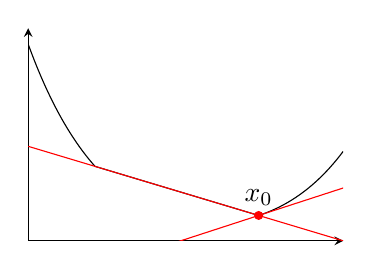
\begin{tikzpicture}
      \begin{axis}[
        ticks=none,
        axis lines=left,
        y=3cm,            % y unit vector
        x=1cm,            % x unit vector
        xmin=-2,
        xmax=2,
        ymin=0.1,
        ymax=1,
        clip=true
        ]
        
        \addplot[mark=none, black, samples=100, domain=-2:2] {max((exp(-x)+exp(x)/2)/8, 0.3 - 0.1*(x))};

        

        \node[circle, inner sep=1, draw=red, fill=red] (x0) at (axis cs:0.926522, 0.2073478) {};
        \node[above] at (x0) {\red{$x_0$}};

        \addplot[mark=none, red, samples=100, domain=-2:2] {0.2073478 - 0.1*(x-0.926522))};
        \addplot[mark=none, red, samples=100, domain=-2:2] {0.2073478 + 0.108366*(x-0.926522))};
        
        % \addplot+[thick, draw=blue, mark=none, fill=blue] coordinates {(-1,0.362777) (1.5, 0.307996) };
        
      \end{axis}
    \end{tikzpicture}
  \end{minipage}


  \vfill

  The scalar product representation of a subdifferential:
  \[
    \partial f(x_0) \defn \set{\hat g\in\Re^n}{f(x) \geq f(x_0)+ \iprod{\hat g}{x-x_0}~\forall x\in \Re^n}
  \]
  
\end{frame}

\begin{frame}{First-Order Optimality}
  
  \textbf{Theorem : } Let $f:\Re^n\to\nRe$ be a convex function. Then,
  \[
    x^\star \in \arg\min_{x\in \Re^n} f(x) \iff 0 \in \partial f(x^\star).
  \]

  \textbf{Proof :} We have 
  \[
    f(y) \geq f(x^\star) + \iprod{0}{y-x^\star} =f(x^\star)
  \]
  for any $y \in \Re^n$ if and only if $0 \in \partial f(x^\star)$. 

  \vfill

\begin{center}
    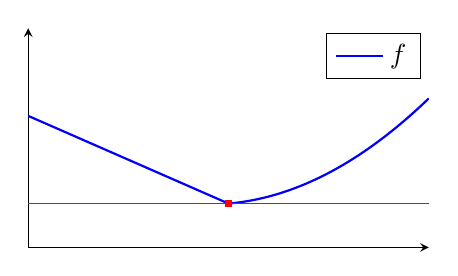
\begin{tikzpicture}
      \begin{axis}[
        axis lines = left,
        ticks={none},
        width=0.55*\textwidth,
        height=0.6*\axisdefaultheight,
        clip=true,
        ymin=-0.5,
        ymax=2
        ]

        \addplot [
        domain=-1:1, 
        samples=100, 
        color=blue,
        thick
        ]
        {max(
          -x,
          0.2*x+x*x
          )};
        \addlegendentry{$f$}

        
        \addplot [
        domain=-1:1, 
        samples=10, 
        color=red,
        ]
        {0};

        \node[draw=red, fill=red, inner sep=1] at (axis cs:0, 0) {};
                
      \end{axis}
    \end{tikzpicture}
  \end{center}

  
\end{frame}



\begin{frame}{Supporting Hyperplanes}

  A \emph{supporting hyperplane} $H=\set{x}{h(x)=\alpha}$, with $h$ a linear function, of a convex set $S$ at a point $x_0 \in \bnd(S)$ is such that $x_0\in H$ and $S\subseteq H^-\defn \set{x}{h(x)\leq \alpha}$.


  \vfill

  \begin{minipage}{0.5\textwidth}
    \centering
    \includesvg[height=4cm]{Supporting_hyperplane1.svg}
  \end{minipage}%
  \hfill
  \begin{minipage}{0.5\textwidth}
    \centering
    \includesvg[height=4cm]{Supporting_hyperplane2.svg}
  \end{minipage}

  \vfill
  {\tiny Figures from Wikimedia Commons}

  \vfill

  \uncover<2->{
    \textbf{Remark : } Supporting hyperplanes are not unique.
  }
\end{frame}



\begin{frame}{Supporting Hyperplanes on Epigraph}

  Let $f : \Re^n\to\nRe$ be a \emph{\acs{lsc} convex} function. Its epigraph $\epi(f)$ is a closed convex set.

  \begin{center}
    \includegraphics[height=3cm]{epigraph/epigraph.pdf}
  \end{center}

  \vfill

  \textbf{Remarks:}
  \begin{itemize}
  \item A non-vertical supporting hyperplane $H$ at $(x_0, f(x_0))$ for $\epi(f)$, say $H=\set{(x, t)\in\Re^n\times \Re}{h(x, t)=\iprod{\hat g}{x}+t\cdot g_0=\beta}$, defines a linear function which satisfies the gradient inequality
  \item<2-> A hyperplane is non-vertical if $g_0\neq 0$
  \item<3-> For a non-vertical hyperplane we may set $g_0=-1$.
  \end{itemize}
  
\end{frame}

\begin{frame}{Supporting Hyperplanes on Epigraph $[\star]$}


  We have that $(x_0, f(x_0)) \in \bnd(\epi(f))$ and hence we can consider all the supporting hyperplanes $H$ of $\epi(f)$. Let $x_0 \in \relint(\dom(f))$. The hyperplane $H$ should not be  ``\emph{vertical}'', i.e.,

  \begin{align*}
    H & = \set{(x, t)\in\Re^n\times \Re}{\iprod{\hat g}{x} - t=\beta}\\
      & = \set{(x, t)\in\Re^n\times \Re}{g(x) - t=\beta}
  \end{align*}
  with $g(x)=\iprod{\hat g}{x}$ a linear function.

  \vfill

  \uncover<2->{
    \textbf{Remarks :}
  }
  \begin{itemize}
  \item<2-> $(x_0, f(x_0))\in H$ implies that $\beta = g(x_0)-f(x_0)$.
  \item<3-> As $(x, f(x)) \in \epi(f)\subseteq H^-$ for all $x \in \dom(f)$, we have
    \[
      g(x) - f(x)\leq \beta = g(x_0)-f(x_0) \iff \emph{f(x_0) + g(x-x_0) \leq f(x)}
    \]
  \end{itemize}

  \vfill

  \uncover<4->{
    \textbf{Note : } If $f$ is differentiable in $x_0$ then $f'(x_0)$ works (shown earlier).
  }
\end{frame}

\begin{frame}{Recall : Separating a Point from an Open Convex Set}

  \begin{minipage}{0.5\textwidth}
    \textbf{Theorem :} Let $C \subseteq \Re^n$ nonempty \emph{open} convex set and $D=\{y\}$ where $y\notin C$. There exists a linear function $\hat f$ such that $\hat f(x) < \hat f(y)$ for all $x\in C$.
    \vspace{2em}
  \end{minipage}%
  \hfill
  \begin{minipage}{0.5\textwidth}
    \centering
    \includegraphics[height=3.5cm]{separating-hyperplane/separating-open-set-from-point.pdf}
  \end{minipage}
  
\end{frame}

\begin{frame}{The Subdifferential is Nonempty}

  Let $f : \Re^n\to\nRe$ be a \acl{lsc} convex function. 

  \textbf{Theorem : } $$x \in \relint(\dom(f)) \implies \partial f(x)\neq \emptyset$$

  \vfill
  
  \textbf{Proof (sketch for $\relint(\dom(f))=\interior(\dom(f))$): }

  \begin{itemize}
  \item Let $C\defn \interior(\epi(f))$, $D=\{(x, f(x))\}$
  \item Let hyperplane $H\defn \set{y\in \Re^n\times \Re}{h(y)=c\defn h(x, f(x))}$ separate $C$ and $D$
  \item As $C\subseteq \set{y\in \Re^n\times \Re}{h(y)<c}$, we have
  \[
    \epi(f) = \cl(C)\subseteq \set{y\in \Re^n\times \Re}{h(y)\leq c}.
  \]
  and $H$ is hence a supporting hyperplane of $\epi(f)$ at $x$
  \item<2-> $H$ is also not vertical, because $x\in \interior(\dom(f))$.
  \end{itemize}

\end{frame}

\section{Conjugate functions}

\begin{frame}{The Conjugate Function}

  We define the \emph{conjugate} of any function $f:\Re^n\to\Re$ as
  \[
    f^\star(y)\defn \sup_{x\in\Re^n} \iprod{y}{x}-f(x).
  \]
  Note that $f^\star$ is by construction \ac{lsc} and convex.

  \vfill

  \begin{center}
    \includesvg[height=4cm]{conjugate-function.svg}
  \end{center}

  \vfill

  \textbf{Fact :} If $f$ is \ac{lsc} and convex, then $f^{\star\star}=f$.
  
\end{frame}

% \begin{frame}{A Special Dual Problem}

%   Recall \emph{weak duality} using increasing functions $\mc F$, i.e.,
%   \[
%     \begin{array}{rlcrl}
%       \inf & f(x)  & \geq & \sup & F(b) \\[0.5em]
%       \st & x\in \dom(f)   & &                       \st & F \in \mc F \\[0.5em]
%            & x \succeq_K b &&    & F(x) \leq f(x), ~~\forall x \in \dom (f).
%     \end{array}
%   \]

%   Recall that $\mc F \defn \set{x \mapsto \iprod{u}{x} - u_0}{u \in K^\star, ~u_0\in \Re}$ almost (bar Slater's condition) ensures strong duality for convex problems.

%   \vfill
%   The dual problem can be recast as

%   \[
%     \begin{array}{rl}
%       \sup & \iprod{u}{b} - u_0 \\[0.5em]
%       \st & \iprod{u}{x} - u_0 \leq f(x) , ~~\forall x \in \dom (f) \\[0.5em]
%            & u \in K^\star, ~u_0\in \Re.
%     \end{array}
%   \]  
  
% \end{frame}

% \begin{frame}{A Special Dual Problem}

%   We have the special dual problem
%   \[
%     \begin{array}{rl}
%       \sup & \iprod{u}{b} - u_0 \\[0.5em]
%       \st & \iprod{u}{x} - u_0 \leq f(x) , ~~\forall x \in \dom (f) \\[0.5em]
%            & u \in K^\star, ~u_0\in \Re.
%     \end{array}
%   \]
%   with the constraints
%   \begin{align*}
%     & \iprod{u}{x} - u_0  \leq f(x) , ~~\forall x \in \dom (f) \\
%     \iff & \iprod{u}{x} - f(x) \leq u_0, ~~\forall x \in \dom (f).
%   \end{align*}
  
%   \vfill

%   \uncover<2->{
%     The function $f^\star(u)\defn \sup_{x\in\Re^n} \iprod{u}{x}-f(x)$ is the \emph{conjugate} of the function $f$. Given $u$ the optimal $u_0 =f^\star(u)$.
%   }

%   \vfill

%   \uncover<3->{
%   \textbf{Special weak duality:}
%   \[
%     d^\star = \sup_{u\in K^\star} \iprod{u}{b} - f^\star(u) \leq \inf_{x\succeq_K b} f(x) \leq f(b)
%   \]
%   }
% \end{frame}


\begin{frame}{Support Functions and Characteristic Functions}

  The \emph{support function} of the set $X$ is
  \[
    \begin{array}{rl}
      \sigma_X(u) \defn \sup & \iprod{u}{x} \\
      \st & x \in X.
    \end{array}
  \]

  It is recognized as the \emph{conjugate} of the \emph{characteristic function} $\chi_X$ of the set $X$, i.e.,
  \[
    \chi_{X}(x) \defn \begin{cases} 0 & {\rm{if}}~x\in X,\\ +\infty & {\rm{if}}~x\notin X. \end{cases}
  \]

  
\end{frame}

\begin{frame}{Examples}

  \textbf{Examples :}
  \begin{itemize}
    \setlength{\itemsep}{1em}
  \item Point : $X=\{x\}$. Then $\sigma_X(u) = \iprod{u}{x}$.
  \item $k$-simplex : $X=\conv(\{v_0, \dots, v_k\})$.
    \[
      \sigma_X(u) = \sup \set{\iprod{u}{\textstyle\sum_{i=0}^k p_i v_i}}{p_i\geq 0, ~\textstyle\sum_{i=0}^k p_i=1} =\textstyle \max_{i\in[0,\dots, k]} \iprod{u}{v_i}.
    \]
  \item Half-space : $X= \set{x\in \Re^n}{\iprod{a}{x}\leq b}$. Then, $\sigma_X(\gamma a) = \gamma b$ for $\gamma \geq 0$ and $+\infty$ otherwise.
  \item Dual norm : $X=\set{x}{\norm{x}\leq 1}$. Then $\sigma_X(u)=\norm{u}_\star$.
  \end{itemize}

  
\end{frame}

\begin{frame}{Support Function of Subdifferential}

  Let $f:\Re^n\to\nRe$ be a \ac{lsc} convex function. Let $x\in\relint(\dom(f))$.

  \vfill

  \textbf{Theorem : } The support function of $\partial f(x)$ is $h(d)\defn \nabla f(x)[d]$.

  
\end{frame}

\begin{frame}{Proof}

  \textbf{Proof [$\star$] :}

  Fix $x\in \relint(\dom(f))$ and $d\in \Re^n$. We need to check $h(d) = \sup \set{\iprod{g}{d}\!}{\!g \in \partial f(x)}$. First, $h(d) \geq \sup \set{\iprod{g}{d}\!}{\!g \in \partial f(x)}$ as
  \[
    \forall g \in \partial f(x), ~ h(d)\defn \lim_{t\downarrow 0} \, \mu(t)\defn (f(x+t d) - f(x))/t \geq \iprod{g}{td}/t = \iprod{g}{d}.
  \]
  Second, the function $h$ is convex with $\dom(h)=\Re^n$ as $f$ is convex and $x\in\relint(\dom(f))$. Thus, $\partial h(d) \neq \emptyset$. Let $g_h\in \partial h(d)$ and $v\in\Re^n$. Note that for all $\tau \geq 0$
  \[
    \tau h(v) = h(\tau v) \geq h(d) + \iprod{g_h}{\tau v - d} \implies h(v)\geq \iprod{g_h}{v} = h(0) + \iprod{g_h}{v},
  \]
  by taking $\tau\to\infty$. Hence, $g_h \in \partial h(0)$. Also for $\tau=0$, we have $\iprod{g_h}{d}\geq h(d)$. As $\mu(t)$ is decreasing with $t\downarrow 0$ for convex $f$ and $g_h \in \partial h(0)$ we have
  \[
    f(y) - f(x) \geq \lim_{t\downarrow 0} \, (f(x + t(y-x))-f(x))/t =  h(y-x) \geq \iprod{g_h}{y-x} \forall x, y \in \dom(f).
  \]
  Therefore, $g_h\in \partial f(x)$ and $\sup\set{\iprod{g}{d}}{g\in\partial f(x)} \geq \iprod{g_h}{d} \geq h(d)$.
  
\end{frame}

\begin{frame}{Subdifferential and Differential}

  \textbf{Theorem :} A convex function $f$ is differentiable at $x$ if and only if $\partial f(x) = \{g\}$. In that case, $g = f'(x)$.

  \vfill
  
  \textbf{Proof [$\star$]:}

  Assume that $\partial f(x)=\{g\}$. The support function of $\partial f(x)$ is $\iprod{g}{d} = \nabla f(x)[d]$. As the directional derivative is a linear function, $f$ is differentiable in $x$. Moreover, $g = f'(x)$. Conversely, if $f$ is differentiable, $\nabla f(x)[d]$ is linear, i.e.\ the support function of a single point. Thus, $\partial f(x)$ is a singleton.
\end{frame}

\begin{frame}{Conjugates and Subdifferentials}

  

  \textbf{Theorem : } Let $f:\Re^n\to\nRe$ be a \ac{lsc} convex function. $$g \in \partial f(x) \iff x \in \partial f^\star(g).$$

  \vfill
  
  \textbf{Proof [$\star$]:}
  By definition we have the subdifferential that
  \begin{align*}
    g\in \partial f(x) \iff & \,f(y) \geq f(x) + \iprod{g}{y-x} \quad \forall y\in\Re^n\\
                       \iff & \iprod{g}{x}-f(x) \geq {\textstyle\sup_{y\in \Re^n}} \iprod{g}{y} -f(y) = f^\star(g) \geq \iprod{g}{x}-f(x).
  \end{align*}
  Hence,
  \(
  g\in \partial f(x) \iff f^\star(g) + f(x) = \iprod{g}{x}.
  \)
  Recall that $f^\star$ is always a convex \ac{lsc} function. Hence likewise,
  \(
  x \in \partial f^\star(g) \iff f^{\star\star}(x) + f^\star(g) = \iprod{x}{g}.
  \)
  The theorem follows from $f^{\star\star}=f$.
\end{frame}


\end{document}
%%% Local Variables:
%%% mode: latex
%%% TeX-master: t
%%% End:
